\documentclass[tikz]{standalone}

\begin{document}

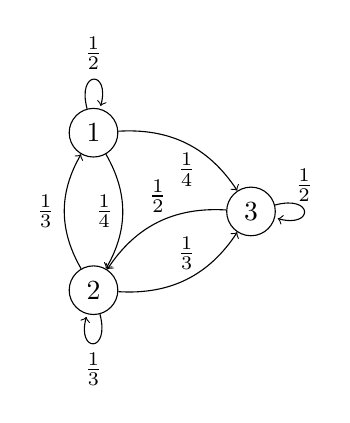
\begin{tikzpicture}
    \node [circle , draw ] (zero) at (0,1) {1};
    \node [circle , draw ] (one) at (0,-1) {2};
    \node [circle , draw ] (two) at (2,0) {3};
    \path[->] (zero) edge [loop above] node {$\frac{1}{2}$} (zero);
    \path[->] (one) edge [loop below] node {$\frac{1}{3}$} (one);
    \path[->] (zero) edge [bend left] node [left] {$\frac{1}{4}$} (one);
    \path[->] (one) edge [bend left] node [left] {$\frac{1}{3}$} (zero);
    \path[->] (zero) edge [bend left] node [below] {$\frac{1}{4}$} (two);
    \path[->] (one) edge [bend right] node [above] {$\frac{1}{3}$} (two);
    \path[->] (two) edge [bend right] node [above] {$\frac{1}{2}$} (one);
    \path[->] (two) edge [loop right] node [above] {$\frac{1}{2}$} (two);
\end{tikzpicture}
\end{document}
